\documentclass{beamer}

\usepackage[utf8]{inputenc}
\usepackage[catalan]{babel}
\usepackage{graphicx}
\usepackage{textpos} 
\usepackage{hyperref}
\usepackage[textfont={small,it}]{caption}

\usetheme{metropolis}

\title[TFG]{\Large{Sistema d'autolocalització per a robots mòbils mitjançant tècniques de visió per computador}\\\hspace{0.05cm}\large{Treball final de grau}}
\author{Joan Rodas Cusidó}
\institute{Facultat Informàtica de Barcelona\\Universitat Politècnica de Catalunya}
\date{20 d'octubre de 2016}

\setbeamertemplate{footline}{%
	\begin{beamercolorbox}[ht=2.25ex,dp=3ex,right]{normal text}%
		\insertframenumber{} / \inserttotalframenumber\hspace*{2ex}
	\end{beamercolorbox}
}

\addtobeamertemplate{frametitle}{}{%
	\begin{textblock*}{100mm}(\textwidth,-0.95cm)
		
\includegraphics[height=0.8cm,width=0.8cm]{logo.png}
	\end{textblock*}
}

\setbeamerfont{footline}{size=\fontsize{7}{11}\selectfont}

\begin{document}

	% TITLE
	\begin{frame}[plain]
		\titlepage
	\end{frame}

	% PROJECT
	\begin{frame}{Projecte}
		\large\textbf{Web}
		\begin{itemize}
			\item Llistat de manga llicenciats en anglès
		\end{itemize}
			\vspace{1em}
			\large\textbf{Aplicació Android}
		\begin{itemize}
			\item Gestionar col·leccions
		\end{itemize}
	\end{frame}

	% HOURS
	\begin{frame}{Distribució hores}
		\begin{itemize}
			\item Disseny/Idea: 2h
			\item Preparació entorn: 2h
			\item Cerca d'informació: +5h
			\item Creació web: 20h
			\item Creació/Disseny BD: 2h
			\item Introducció dades a la BD: massa temps :-)
			\item Programació app: ~8h
			\item Preparació defensa: 4h
		\end{itemize}
	\end{frame}

	% LICENSE
	\begin{frame}{Llicència}
		GNU GPL v3.0
		\begin{itemize}
			\item Codi obert
			\item Còpia
			\item Distribució (comercial o no)
			\item Modificació
			\item Mateixa llicència 
		\end{itemize}
	\end{frame}

	% WHERE
	\begin{frame}{On trobar-ho?}

		\large\textbf{Web/Servidor}
		\begin{itemize}
			\item Codi: Github (\href{https://github.com/wildux/licensedmanga-web}{github.com/wildux/licensedmanga-web})
			\item Web: \url{http://licensedmanga.com}
		\end{itemize}
			\vspace{1em}
			\large\textbf{Aplicació d'Android}
		\begin{itemize}
			\item Codi: Github (\href{https://github.com/wildux/licensedmanga-app}{github.com/wildux/licensedmanga-app})
			\item Traducció: Localize (\href{http://www.localize.im/v/rg}{www.localize.im/v/rg})
		\end{itemize}

	\end{frame}

	% WHY
	\begin{frame}{Per què?}

		\begin{columns}[t]
			\column{0.5\textwidth}
			\large\textbf{Anime News Network}
			\begin{itemize}
				\small\item Llistat poc amigable
				\item Sense informació sobre dates de llançament
			\end{itemize}
			\vspace{1em}
			\large\textbf{Manga Updates}
			\begin{itemize}
				\small\item Llistat poc amigable
				\item Sense informació sobre dates de llançament
			\end{itemize}
			\column{0.5\textwidth}
			\large\textbf{Whakoom}
			\begin{itemize}
				\small\item Poques obres en anglès (pàgina en castellà)
				\item Pàgina de còmics en general
			\end{itemize}
			\vspace{1em}
			\large\textbf{MyAnimeList}
			\begin{itemize}
				\small\item Pensada per scans
			\end{itemize}
		\end{columns}

	\end{frame}


	%%%%%%%%%%%%%%%%%%%%%%%%%%%%%
	% 			WEB				%
	%%%%%%%%%%%%%%%%%%%%%%%%%%%%%

	\begin{frame}
		\section{Web}
	\end{frame}

	% SERIES
	\begin{frame}
	\frametitle{Web - Sèries}
		\begin{figure}
			\centering
			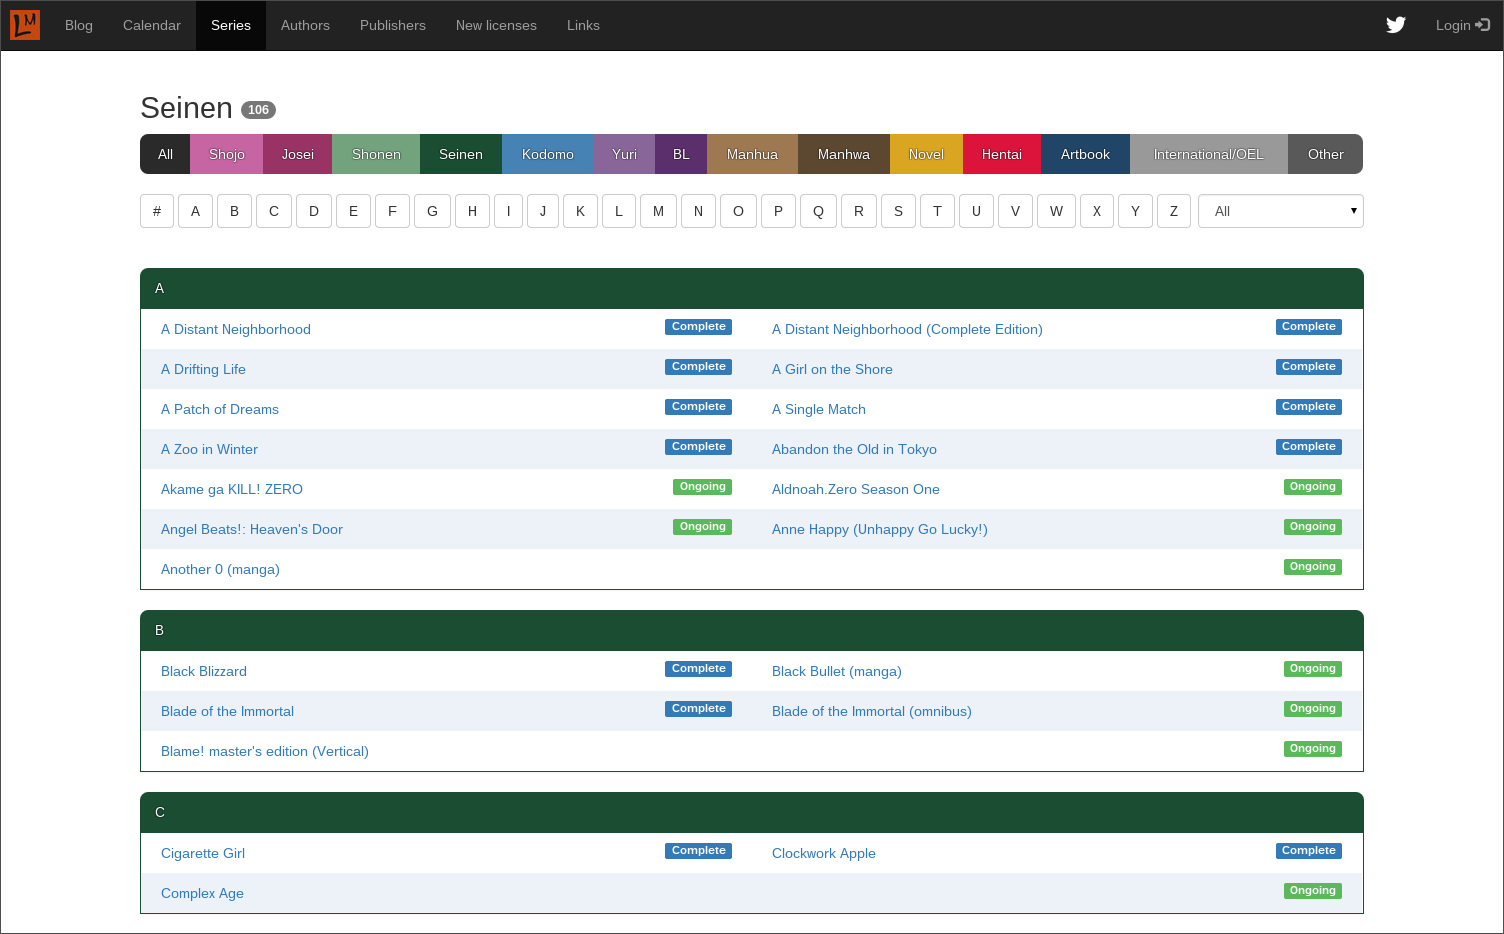
\includegraphics[width=1\textwidth]{series.png}
			\caption{Llistat sèries (Seinen)}
		\end{figure}
	\end{frame}

	% SERIE INFO
	\begin{frame}
	\frametitle{Web - Informació sèrie}
		\begin{figure}
			\centering
			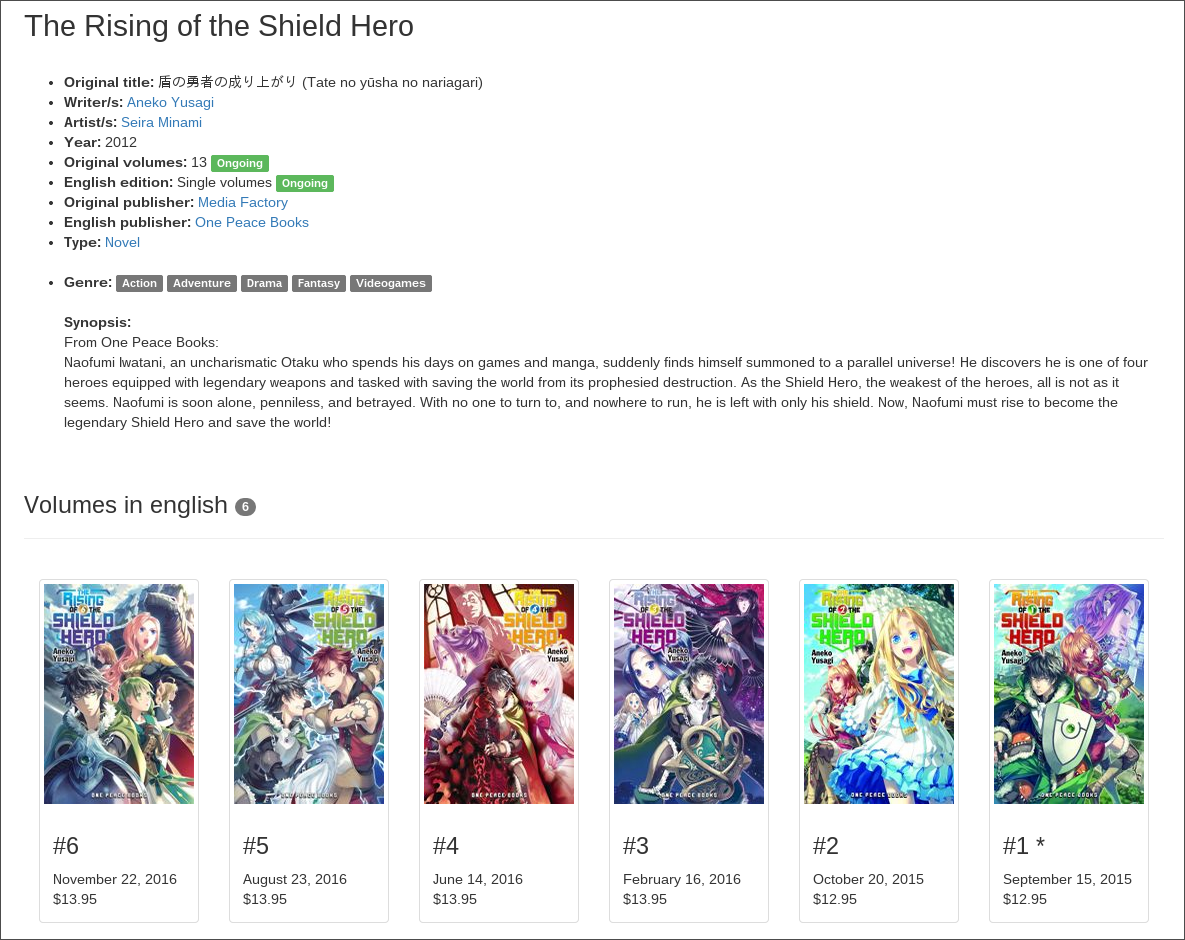
\includegraphics[scale=0.20]{shield.png}
			\caption{The Rising of the Shield Hero}
		\end{figure}
	\end{frame}

	% AUTHORS
	\begin{frame}
	\frametitle{Web - Autors}
		\begin{figure}
			\centering
			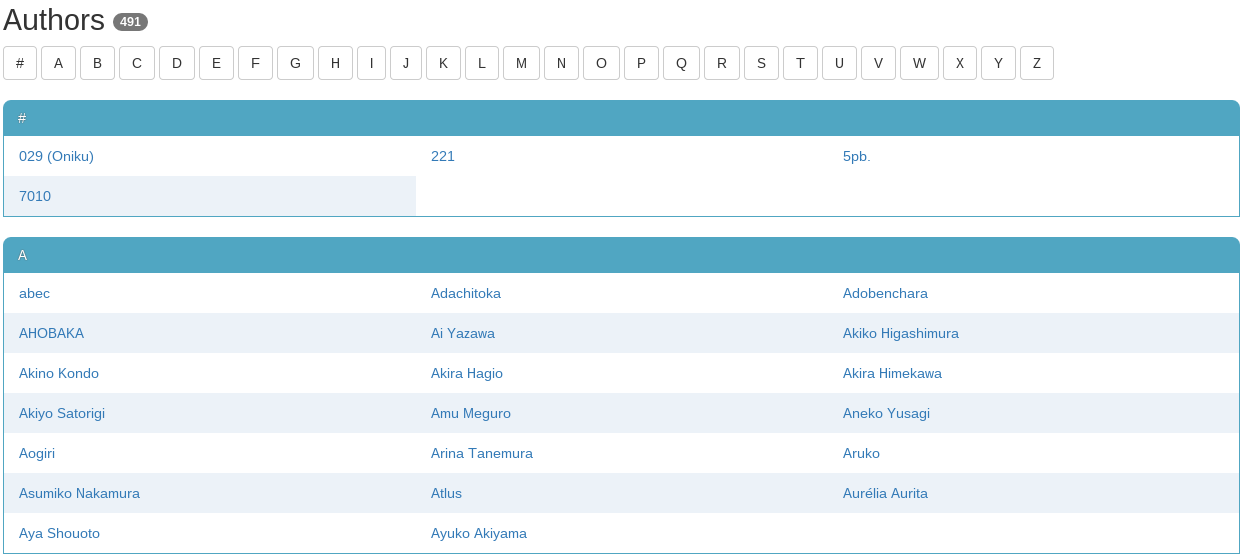
\includegraphics[width=1\textwidth]{authors.png}
			\caption{Llistat autors}
		\end{figure}
	\end{frame}

	% PUBLISHERS
	\begin{frame}
	\frametitle{Web - Editorials}
		\begin{figure}
			\centering
			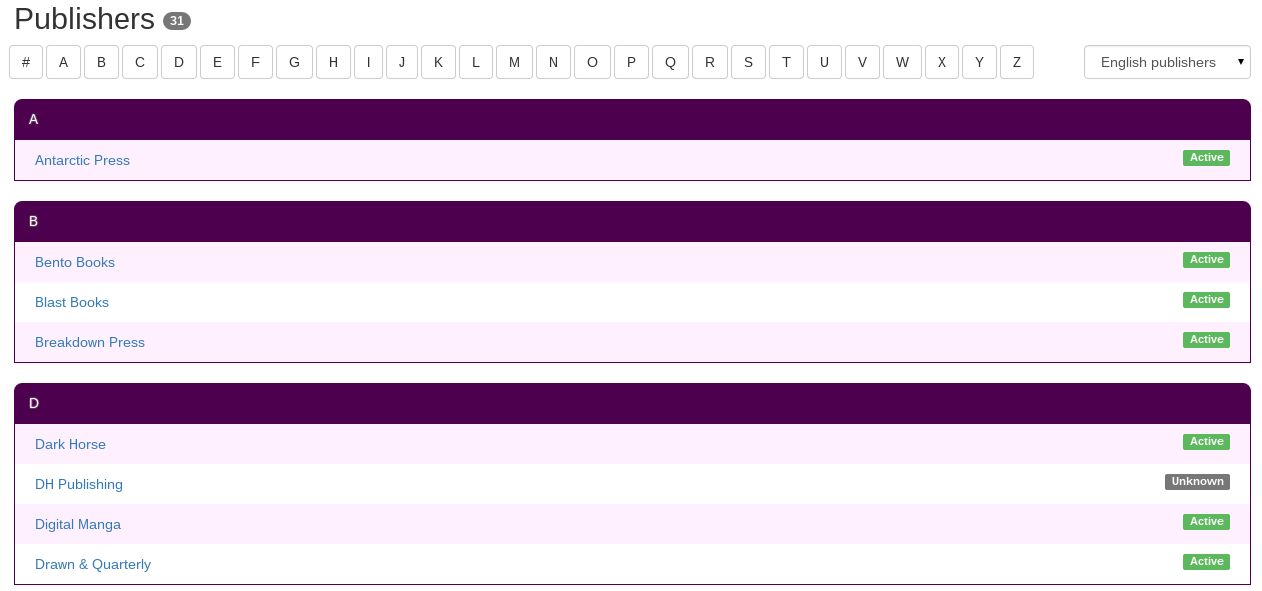
\includegraphics[width=1\textwidth]{publishers.png}
			\caption{Llistat editorials}
		\end{figure}
	\end{frame}

	% CALENDAR
	\begin{frame}
	\frametitle{Web - Calendari}
		\begin{figure}
			\centering
			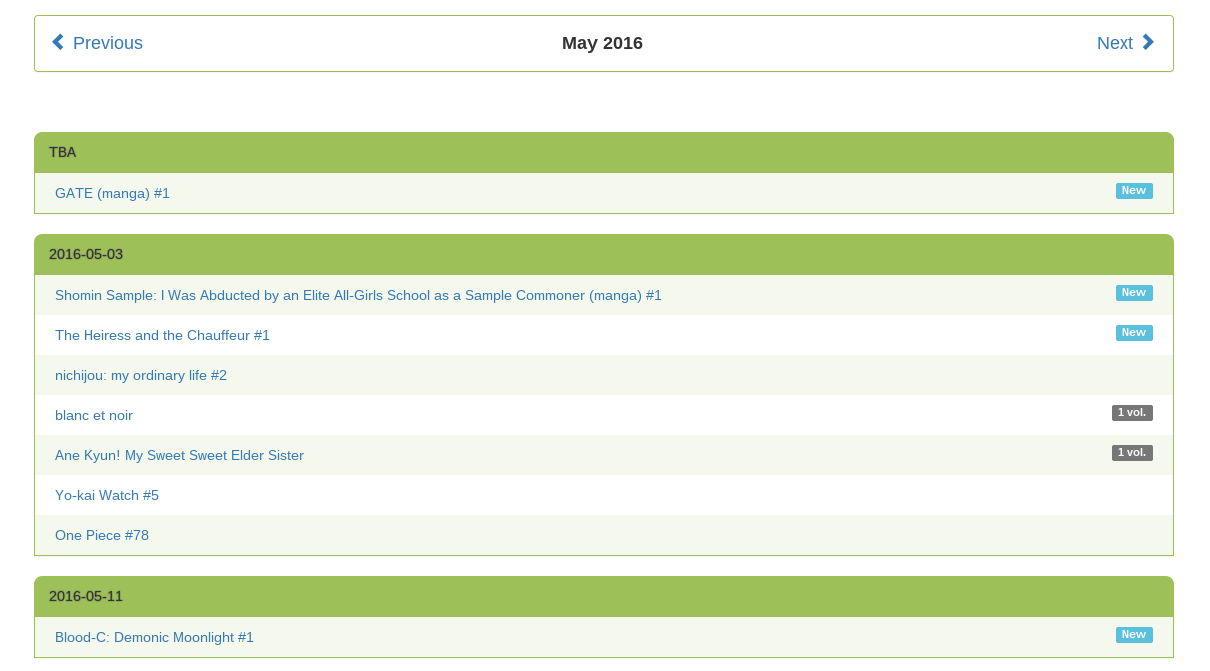
\includegraphics[width=1\textwidth]{calendar.png}
			\caption{Calendari de llançaments}
		\end{figure}
	\end{frame}

	% NEW LICENSES
	\begin{frame}
	\frametitle{Web - Noves llicències}
		\begin{figure}
			\centering
			
\includegraphics[scale=0.4]{new_licenses.png}
			\caption{Noves llicències}
		\end{figure}
	\end{frame}

	%%%%%%%%%%%%%%%%%%%%%%%%%%%%%
	% 			APP				%
	%%%%%%%%%%%%%%%%%%%%%%%%%%%%%

	\begin{frame}
		\section{Aplicació d'Android}
	\end{frame}

	% MAIN MENU
	\begin{frame}
	\frametitle{App - Menú principal}
		\begin{figure}
			\centering
			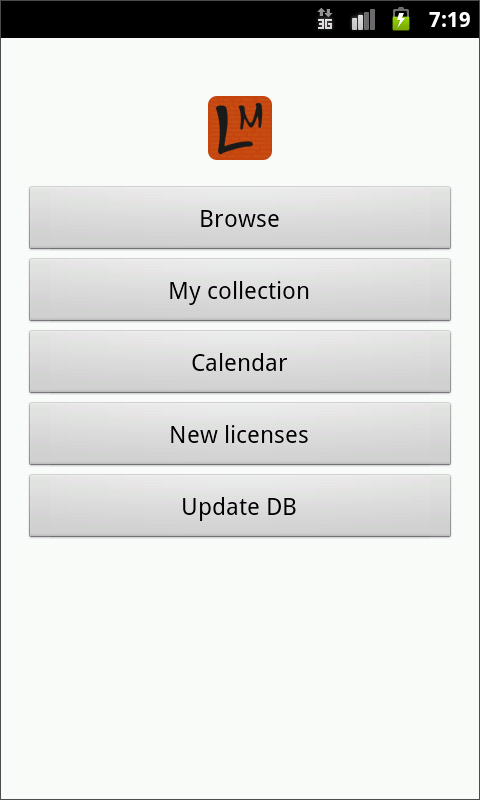
\includegraphics[scale=0.23]{main_menu.png}
			\caption{Menú principal}	
		\end{figure}
	\end{frame}

	% BROWSE
	\begin{frame}
	\frametitle{App - Cercar sèries}
		\begin{figure}
			\centering
			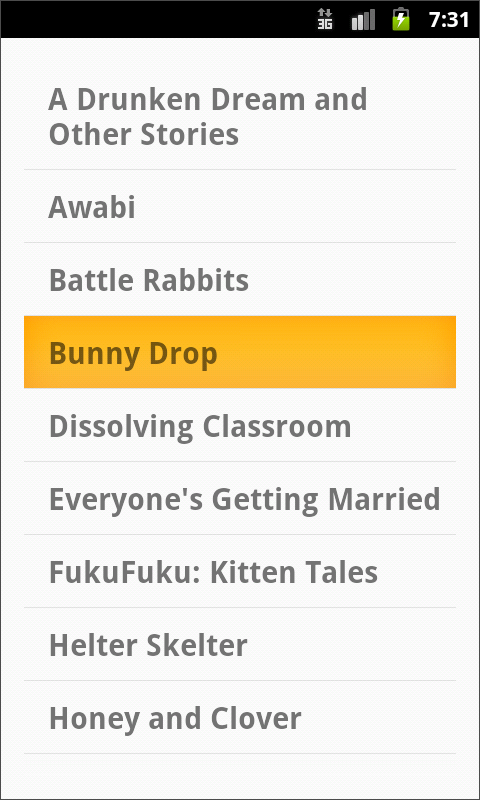
\includegraphics[scale=0.23]{series_list.png}\hspace*{3ex}
			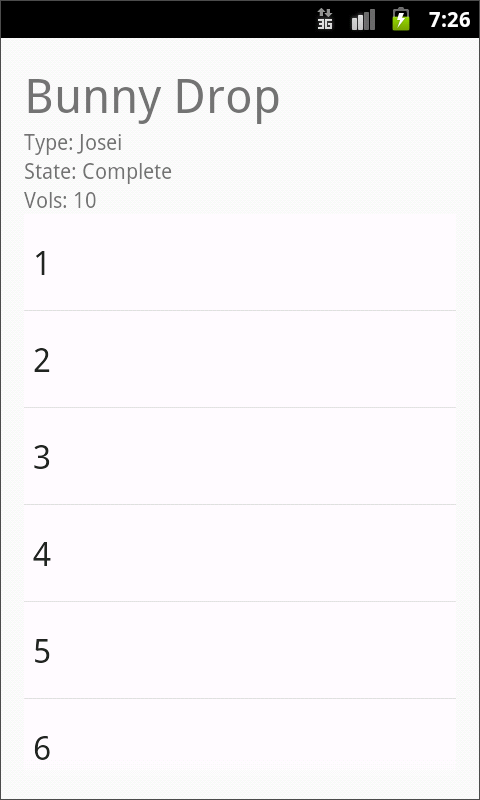
\includegraphics[scale=0.23]{serie.png}
			\caption{Llistat de josei / Informació Bunny Drop}	
		\end{figure}
	\end{frame}

	% COLLECTION MENU
	\begin{frame}
	\frametitle{App - Col·lecció (I)}
		\begin{figure}
			\centering
			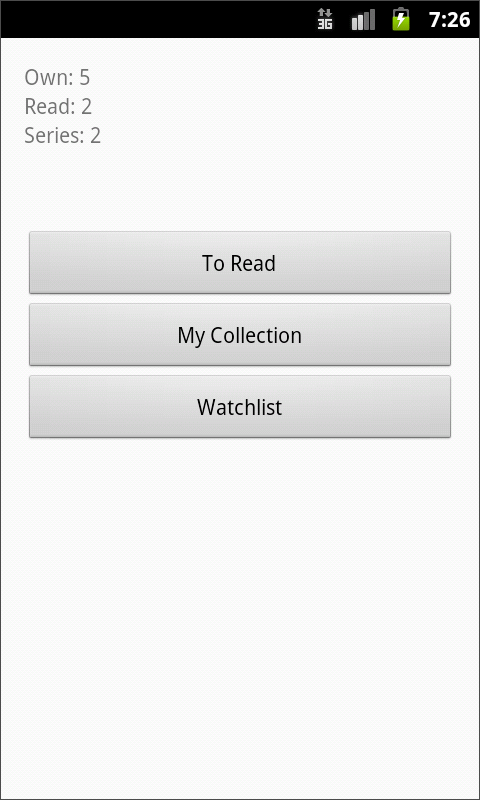
\includegraphics[scale=0.23]{collection_menu.png}\hspace*{3ex}	
			
\includegraphics[scale=0.23]{collection.png}
			\caption{Menú col·lecció / Veure col·lecció}
		\end{figure}
	\end{frame}

	% MY COLLECTION
	\begin{frame}
	\frametitle{App - Col·lecció (II)}
		\begin{figure}
			\centering
			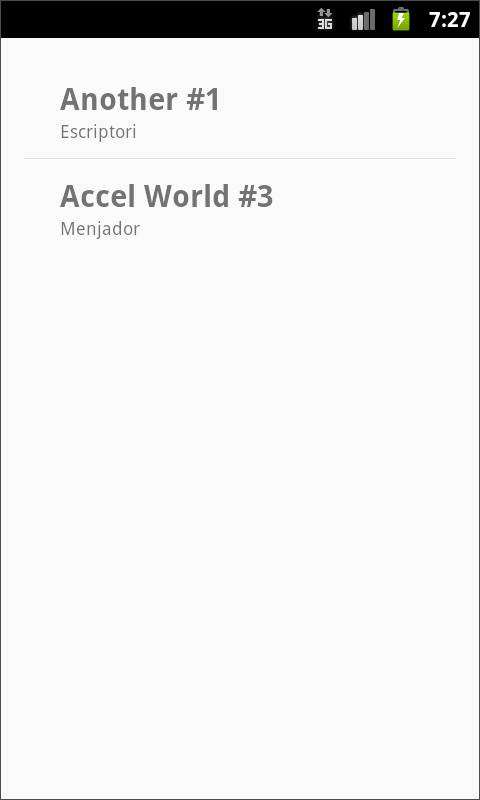
\includegraphics[scale=0.23]{to_read.png}\hspace*{3ex}
			
\includegraphics[scale=0.23]{watchlist.png}
			\caption{Volums per llegir / Watchlist}
		\end{figure}
	\end{frame}

	% CALENDAR
	\begin{frame}
	\frametitle{App - Calendari}
		\begin{figure}
			\centering
			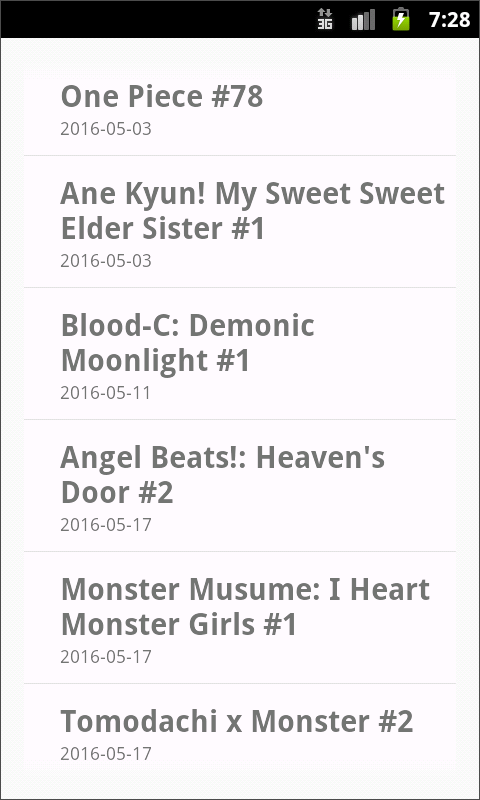
\includegraphics[scale=0.23]{new_releases.png}
			\caption{Últims llançaments}
		\end{figure}
	\end{frame}

	% NEW LICENSES
	\begin{frame}
	\frametitle{App - Noves llicències}
		\begin{figure}
			\centering
			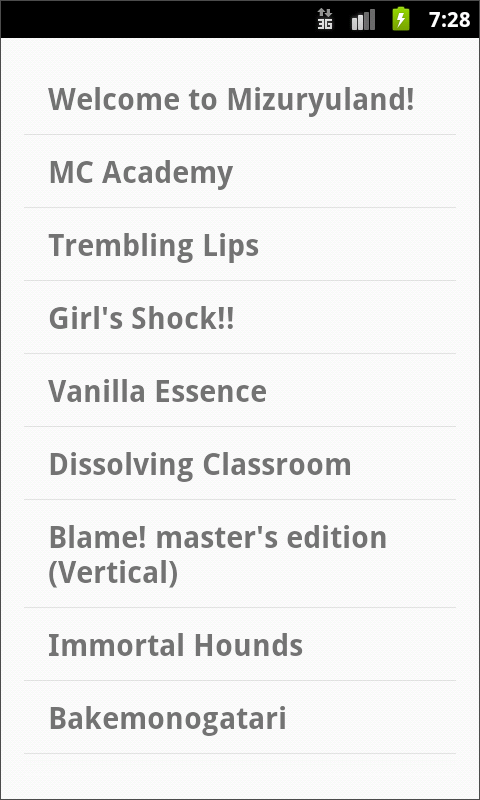
\includegraphics[scale=0.23]{app_new_licenses.png}
			\caption{Noves llicències}
		\end{figure}
	\end{frame}

	% END
	\begin{frame}{Possibles millores}
		\begin{itemize}
			\item Puntuacions/Rankings
			\item Ressenyes
			\item Component social (compartir col·leccions)
			\item Enllaços compra (Amazon)
			\item Cerca mitjançant introducció text
		\end{itemize}
	\end{frame}


\end{document}
